\documentclass[border=10pt]{standalone}
\usepackage{tikz}
\usetikzlibrary{shapes.geometric, arrows.meta, positioning, fit, backgrounds, calc, decorations.pathreplacing, shadows.blur}

\definecolor{hwgreen}{HTML}{2E7D32}
\definecolor{mqttblue}{HTML}{1565C0}
\definecolor{cloudpurple}{HTML}{6A1B9A}
\definecolor{backorange}{HTML}{E65100}
\definecolor{dbred}{HTML}{BF360C}
\definecolor{aiteal}{HTML}{00838F}
\definecolor{appblue}{HTML}{0277BD}
\definecolor{flowgray}{HTML}{37474F}

\begin{document}
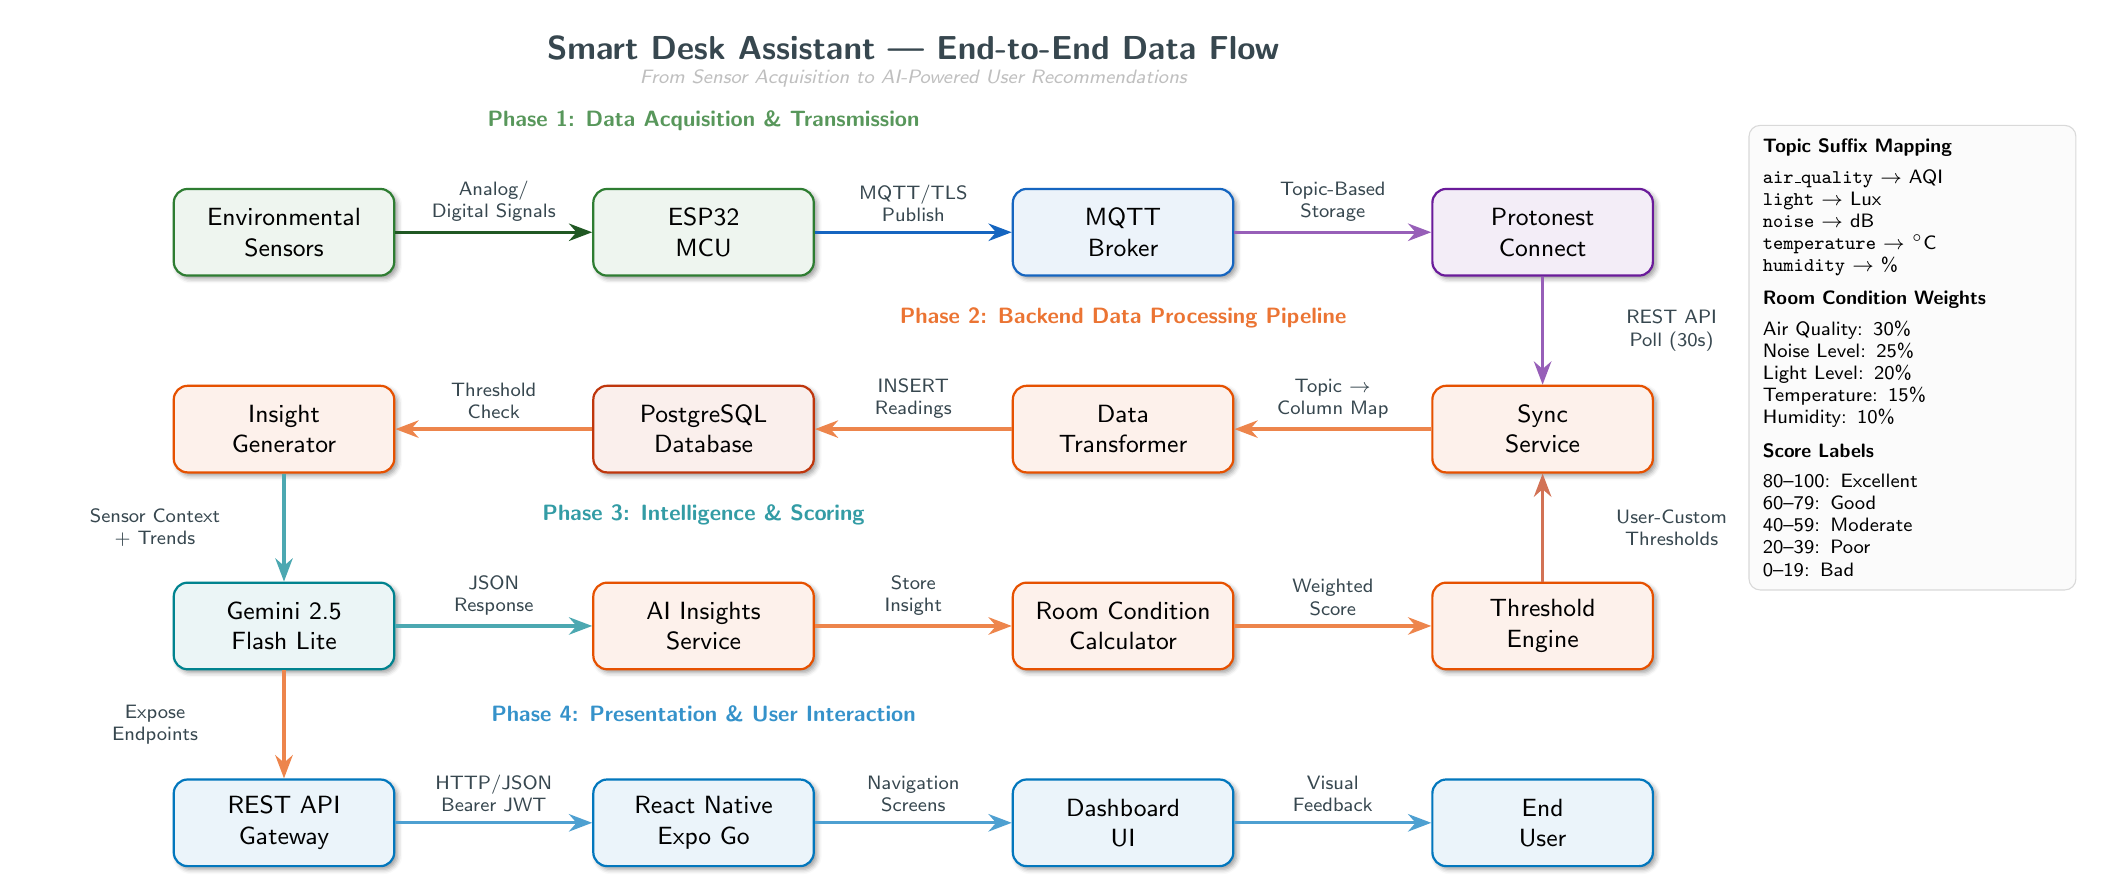
\begin{tikzpicture}[
    block/.style={
        rectangle, rounded corners=5pt, draw=#1, fill=#1!8,
        minimum width=2.8cm, minimum height=1.1cm, align=center,
        font=\small\sffamily, line width=0.8pt,
        blur shadow={shadow blur steps=4, shadow xshift=0.4mm, shadow yshift=-0.4mm}
    },
    block/.default=flowgray,
    flowarrow/.style={
        -Stealth, line width=1.2pt, color=flowgray
    },
    flowlabel/.style={
        font=\scriptsize\sffamily, color=flowgray, align=center, text width=3cm
    },
    phaselabel/.style={
        font=\footnotesize\sffamily\bfseries, color=#1!80, align=center
    },
    phaselabel/.default=flowgray
]

% ============================================================
% Row 1: Hardware Data Acquisition
% ============================================================

\node[block=hwgreen] (sensors) at (0, 0) {Environmental\\Sensors};
\node[block=hwgreen, right=2.5cm of sensors] (esp32) {ESP32\\MCU};
\node[block=mqttblue, right=2.5cm of esp32] (mqtt) {MQTT\\Broker};
\node[block=cloudpurple, right=2.5cm of mqtt] (protonest) {Protonest\\Connect};

\draw[flowarrow, hwgreen!70!black] (sensors) -- node[above, flowlabel] {Analog/\\Digital Signals} (esp32);
\draw[flowarrow, mqttblue] (esp32) -- node[above, flowlabel] {MQTT/TLS\\Publish} (mqtt);
\draw[flowarrow, cloudpurple!70] (mqtt) -- node[above, flowlabel] {Topic-Based\\Storage} (protonest);

% Phase label
\node[phaselabel=hwgreen, above=0.6cm of esp32] {Phase 1: Data Acquisition \& Transmission};

% ============================================================
% Row 2: Backend Processing
% ============================================================

\node[block=backorange] (sync) at ($(protonest)+(0,-2.5)$) {Sync\\Service};
\node[block=backorange, left=2.5cm of sync] (transform) {Data\\Transformer};
\node[block=dbred, left=2.5cm of transform] (db) {PostgreSQL\\Database};
\node[block=backorange, left=2.5cm of db] (insight_eng) {Insight\\Generator};

\draw[flowarrow, cloudpurple!70] (protonest.south) -- node[right, flowlabel] {REST API\\Poll (30s)} (sync.north);
\draw[flowarrow, backorange!70] (sync) -- node[above, flowlabel] {Topic $\rightarrow$\\Column Map} (transform);
\draw[flowarrow, backorange!70] (transform) -- node[above, flowlabel] {INSERT\\Readings} (db);
\draw[flowarrow, backorange!70] (db) -- node[above, flowlabel] {Threshold\\Check} (insight_eng);

% Phase label
\node[phaselabel=backorange, above=0.6cm of transform] {Phase 2: Backend Data Processing Pipeline};

% ============================================================
% Row 3: Intelligence Layer
% ============================================================

\node[block=aiteal] (gemini) at ($(insight_eng)+(0, -2.5)$) {Gemini 2.5\\Flash Lite};
\node[block=backorange, right=2.5cm of gemini] (ai_svc) {AI Insights\\Service};
\node[block=backorange, right=2.5cm of ai_svc] (room) {Room Condition\\Calculator};
\node[block=backorange, right=2.5cm of room] (thresh) {Threshold\\Engine};

\draw[flowarrow, aiteal!70] (gemini) -- node[above, flowlabel] {JSON\\Response} (ai_svc);
\draw[flowarrow, backorange!70] (ai_svc) -- node[above, flowlabel] {Store\\Insight} (room);
\draw[flowarrow, backorange!70] (room) -- node[above, flowlabel] {Weighted\\Score} (thresh);

% Connect insight_eng down to gemini
\draw[flowarrow, aiteal!70] (insight_eng.south) -- node[left, flowlabel] {Sensor Context\\+ Trends} (gemini.north);

% Connect thresh back up to db
\draw[flowarrow, dbred!70] (thresh.north) -- node[right, flowlabel] {User-Custom\\Thresholds} (db.south -| thresh.north);

% Phase label
\node[phaselabel=aiteal, above=0.6cm of ai_svc] {Phase 3: Intelligence \& Scoring};

% ============================================================
% Row 4: Presentation
% ============================================================

\node[block=appblue] (api) at ($(gemini)+(0, -2.5)$) {REST API\\Gateway};
\node[block=appblue, right=2.5cm of api] (app) {React Native\\Expo Go};
\node[block=appblue, right=2.5cm of app] (dash) {Dashboard\\UI};
\node[block=appblue, right=2.5cm of dash] (user) {End\\User};

\draw[flowarrow, appblue!70] (api) -- node[above, flowlabel] {HTTP/JSON\\Bearer JWT} (app);
\draw[flowarrow, appblue!70] (app) -- node[above, flowlabel] {Navigation\\Screens} (dash);
\draw[flowarrow, appblue!70] (dash) -- node[above, flowlabel] {Visual\\Feedback} (user);

% Connect api up
\draw[flowarrow, backorange!70] (gemini.south) -- node[left, flowlabel] {Expose\\Endpoints} (api.north);

% Phase label
\node[phaselabel=appblue, above=0.6cm of app] {Phase 4: Presentation \& User Interaction};

% ============================================================
% Vertical annotations (right side)
% ============================================================

\node[rectangle, rounded corners=4pt, draw=gray!30, fill=gray!3,
      text width=3.8cm, align=left, font=\scriptsize\sffamily, inner sep=5pt,
      anchor=north west]
      at ($(protonest.north east)+(1.2, 0.8)$) {
    \textbf{Topic Suffix Mapping}\\[3pt]
    \texttt{air\_quality} $\rightarrow$ AQI\\
    \texttt{light} $\rightarrow$ Lux\\
    \texttt{noise} $\rightarrow$ dB\\
    \texttt{temperature} $\rightarrow$ $^{\circ}$C\\
    \texttt{humidity} $\rightarrow$ \%\\[4pt]
    \textbf{Room Condition Weights}\\[3pt]
    Air Quality: 30\%\\
    Noise Level: 25\%\\
    Light Level: 20\%\\
    Temperature: 15\%\\
    Humidity: 10\%\\[4pt]
    \textbf{Score Labels}\\[3pt]
    80--100: Excellent\\
    60--79: Good\\
    40--59: Moderate\\
    20--39: Poor\\
    0--19: Bad
};

% ============================================================
% Title
% ============================================================

\node[font=\large\sffamily\bfseries, color=flowgray, anchor=south]
    at ($(sensors.north west)!0.5!(protonest.north east) + (0, 1.5)$)
    {Smart Desk Assistant --- End-to-End Data Flow};

\node[font=\scriptsize\sffamily\itshape, color=gray!50, anchor=south]
    at ($(sensors.north west)!0.5!(protonest.north east) + (0, 1.15)$)
    {From Sensor Acquisition to AI-Powered User Recommendations};

\end{tikzpicture}
\end{document}
